\chapter{Experiments and Result Analysis}
\label{cha:experiments}

\section{Experimental Dataset Introduction}
\label{sec:experiments:dataset}

The foundation of this research is a comprehensive dataset, referred to as \texttt{Dataset\_1}, captured from a multi-axis CNC machine tool. This dataset is designed to reflect real-world manufacturing scenarios, encompassing both normal operational states and several distinct, commonly encountered fault conditions.

\subsection{Data Sources and Sensor Signals}
The data was collected from a multi-axis CNC machine tool's control system, capturing comprehensive operational parameters during various machining processes. The dataset comprises multivariate time-series data with 14 distinct feature channels, which provide a holistic view of the machine's operational state and health condition. These features include:

\begin{itemize}
    \item \textbf{Control Deviation Signals}: \texttt{ControlDifference\_X}, \texttt{ControlDifference\_Y}, \texttt{ControlDifference\_A}, \texttt{ControlDifference\_B}, representing control system deviations for each axis
    \item \textbf{Current Measurements}: \texttt{Cur\_Y}, \texttt{Cur\_A}, \texttt{Cur\_B}, \texttt{Cur\_SP}, capturing motor current characteristics for Y-axis, A-axis, B-axis and setpoint current
    \item \textbf{Position Commands}: \texttt{Pos\_X\_cmd}, \texttt{Pos\_A\_cmd}, representing position command signals for X-axis and A-axis
    \item \textbf{Contour Deviations}: \texttt{ContourDeviation\_X}, \texttt{ContourDeviation\_Y},\newline
    \hspace*{1.5em}\texttt{ContourDeviation\_A},\newline
    representing contour machining deviations for X-axis, Y-axis, and A-axis
\end{itemize}

This comprehensive feature set captures the machine's dynamic behavior across multiple dimensions, including control system performance, electrical characteristics, mechanical motion precision, and machining quality. The multi-modal nature of the data enables the detection of various fault patterns and anomalies that manifest across different aspects of machine operation. The time series data is collected at a 2ms sampling interval, ensuring high-precision monitoring of the machine's dynamic behavior. Note that \texttt{time} and \texttt{LineNumber} are used for time series indexing but are not considered as input features for the model.

\subsection{Fault Categories and Physical Meanings}
The dataset is categorized into one normal class and three primary fault classes. Each fault type has a distinct physical manifestation that impacts machining quality:
\begin{itemize}
    \item \textbf{Normal (Good)}: Represents the machine operating under ideal conditions without any detectable faults. This serves as the baseline for anomaly detection.
    \item \textbf{Backlash}: A common mechanical error in motion systems involving gears or lead screws. It refers to the clearance or "play" between mechanical components, which results in lost motion and positioning inaccuracies when the axis of movement is reversed.
    \item \textbf{Ball Screw Degradation (BS)}: This fault signifies wear, friction, or other forms of degradation in the ball screw mechanism, which is responsible for converting rotational motion into precise linear motion. Such degradation can lead to reduced accuracy and surface finish defects.
    \item \textbf{Jerk Anomaly}: Refers to an abnormally high rate of change in acceleration. In a CNC machine, this can be caused by abrupt changes in tool path, control signal instability, or mechanical vibrations, indicating unsmooth operation that can compromise the workpiece.
\end{itemize}

Our fault diagnosis system processes 12 distinct fault categories as defined in the label set:
\begin{align}
\mathcal{L} = \{\text{good}, \text{JERK\_A}, \text{BACKLASH\_X}, \text{JERK\_ALL}, \nonumber \\
\text{ALL\_processed}, \text{JERK\_X}, \text{BACKLASH\_Y}, \text{BS\_XY}, \nonumber \\
\text{BS\_X}, \text{JERK\_Y}, \text{JERK\_B}, \text{BS\_Y}\}
\end{align}

\subsection{Class Distribution and Imbalance}
A critical characteristic of this dataset is the significant class imbalance, which is typical for real-world fault diagnosis scenarios where faulty states are much rarer than normal operation. Figure~\ref{fig:class_distribution_merged} illustrates the distribution of data samples across the four categories.

\begin{figure}[h!]
    \centering
    \includegraphics[width=0.8\textwidth]{../PROJECT/imgs/class_distribution_merged.png}
    \caption{Distribution of samples across different classes, highlighting the significant data imbalance between the 'good' class and the various fault classes.}
    \label{fig:class_distribution_merged}
\end{figure}

The 'good' class contains a substantially larger number of samples compared to any of the fault classes. This imbalance poses a challenge for training a classification model, as the model might develop a bias towards the majority class. Therefore, addressing this imbalance through techniques like data augmentation, resampling, or specialized loss functions is a key consideration in the model development process, which has been discussed in Chapter~\ref{cha:hybrid_model}.

\section{Experimental Environment and Parameter Settings}
\label{sec:experiments:environment_parameters}

This section provides a comprehensive overview of the experimental setup, including the hardware and software environment as well as the detailed parameter configurations used throughout the experiments.

\subsection{Hardware Environment}
\label{subsec:hardware_environment}

The experiments were conducted on a high-performance computing system optimized for deep learning tasks. The hardware specifications are as follows:

\begin{itemize}
    \item \textbf{CPU}: Intel or AMD multi-core processor with sufficient computational capacity for data preprocessing and model management
    \item \textbf{GPU}: NVIDIA GPU with CUDA support for accelerated deep learning training (when available)
    \item \textbf{Memory}: Minimum 16GB RAM to handle large datasets and model parameters
    \item \textbf{Storage}: SSD storage for fast data access and model checkpointing
\end{itemize}

The system automatically detects and utilizes available hardware acceleration, supporting CUDA for NVIDIA GPUs, MPS (Metal Performance Shaders) for Apple Silicon, and falls back to CPU computation when necessary. Mixed precision training is enabled on CUDA-compatible devices to optimize memory usage and training speed.

\subsection{Software Environment}
\label{subsec:software_environment}

The experimental framework is implemented using the following software stack:

\begin{itemize}
    \item \textbf{Operating System}: Cross-platform support (Linux, macOS, Windows)
    \item \textbf{Python Version}: Python 3.8 or higher
    \item \textbf{Deep Learning Framework}: PyTorch 1.12+ with CUDA support
    \item \textbf{Scientific Computing}: NumPy 1.21+, SciPy 1.7+
    \item \textbf{Data Processing}: Pandas 1.3+ for data manipulation and analysis
    \item \textbf{Machine Learning}: Scikit-learn 1.0+ for preprocessing and evaluation metrics
    \item \textbf{Visualization}: Matplotlib 3.5+ and Seaborn for result visualization
    \item \textbf{Additional Libraries}: PyWavelets for wavelet transform features, tqdm for progress tracking
\end{itemize}

\subsection{Model Hyperparameters}
\label{subsec:model_hyperparameters}

The TransformerLSTMModel configuration was carefully optimized through extensive experimentation. Table~\ref{tab:hyperparameters} presents the key hyperparameters used in our experiments.

\begin{table}[htbp]
\centering
\caption{Model Hyperparameters and Training Configuration}
\label{tab:hyperparameters}
\begin{tabular}{|l|c|l|}
\hline
\textbf{Parameter Category} & \textbf{Parameter} & \textbf{Value} \\
\hline
\multirow{4}{*}{Data Configuration} & Input Feature Dimension & 14 \\
 & Sequence Length (Window Size) & 64 \\
 & Number of Classes & 12 \\
 & Train/Validation/Test Split & 70\%/15\%/15\% \\
\hline
\multirow{4}{*}{Transformer Settings} & Hidden Dimension & 336 \\
 & Number of Layers & 3 \\
 & Number of Attention Heads & 2 \\
 & Dropout Rate & 0.22 \\
\hline
\multirow{3}{*}{LSTM Configuration} & Hidden Units & 336 \\
 & Number of Layers & 2 \\
 & Bidirectional & True \\
\hline
\multirow{6}{*}{Training Parameters} & Batch Size & 64 \\
 & Maximum Epochs & 150 \\
 & Learning Rate & 0.0006 \\
 & Weight Decay & $6 \times 10^{-5}$ \\
 & Early Stopping Patience & 30 \\
 & Random Seed & 42 \\
\hline
\multirow{3}{*}{Learning Rate Schedule} & Warmup Epochs & 10 \\
 & Warmup Start LR & $1.8 \times 10^{-5}$ (3\% of base LR) \\
 & Cosine Annealing & Enabled \\
\hline
\multirow{3}{*}{Optimization Features} & Mixed Precision Training & Enabled (CUDA only) \\
 & Data Augmentation & Enabled \\
 & Gradient Clipping & Adaptive \\
\hline
\end{tabular}
\end{table}

\subsection{Data Preprocessing Parameters}
\label{subsec:preprocessing_parameters}

The data preprocessing pipeline employs the following configuration:

\begin{itemize}
    \item \textbf{Normalization}: RobustScaler applied channel-wise to handle outliers
    \item \textbf{Sliding Window}: 64-step windows with random sampling for longer sequences
    \item \textbf{Maximum Samples per File}: 800 windows for computational efficiency
    \item \textbf{Data Augmentation Techniques}:
    \begin{itemize}
        \item Amplitude scaling: factors drawn from $\mathcal{U}(0.85, 1.15)$
        \item Gaussian noise injection: $\sigma = 0.01$ of signal standard deviation
        \item Channel dropout: 30\% probability for robustness testing
    \end{itemize}
\end{itemize}

\subsection{Loss Function and Class Balancing}
\label{subsec:loss_class_balancing}

To address the significant class imbalance in the dataset, the following strategies were implemented:

\begin{itemize}
    \item \textbf{Loss Function}: Focal Loss with $\gamma = 2.0$ to focus on hard examples
    \item \textbf{Class Weights}: Automatically computed inverse frequency weights
    \item \textbf{Sampling Strategy}: Balanced sampling during training to ensure equal representation
\end{itemize}

The experimental configuration ensures reproducibility through fixed random seeds (42) and deterministic CUDA operations, while the adaptive hardware detection provides optimal performance across different computing environments.

\section{Evaluation Metrics}
\label{sec:experiments:metrics}

To comprehensively assess the performance of our Transformer-LSTM Model in the context of fault diagnosis, we employ a diverse set of evaluation metrics \citep{hastie2009elements, he2009learning}. These metrics are specifically chosen to address the challenges posed by the class imbalanced nature of our dataset and to provide insights into different aspects of model performance \citep{krawczyk2016learning, chawla2002smote}. This section defines each metric, explains its calculation methodology, and justifies its relevance for fault diagnosis applications.

\subsection{Primary Classification Metrics}
\label{subsec:primary_metrics}

\subsubsection{Accuracy}
\label{subsubsec:accuracy}

Accuracy represents the most intuitive performance measure, defined as the proportion of correctly classified samples out of the total number of samples:

\begin{equation}
\text{Accuracy} = \frac{\text{Number of Correct Predictions}}{\text{Total Number of Predictions}} = \frac{TP + TN}{TP + TN + FP + FN}
\end{equation}

where $TP$, $TN$, $FP$, and $FN$ represent True Positives, True Negatives, False Positives, and False Negatives, respectively.

However, in the context of our fault diagnosis dataset, accuracy can be misleading due to significant class imbalance \citep{he2009learning, krawczyk2016learning}. As demonstrated in Figure~\ref{fig:class_distribution_merged}, the ``good'' class dominates the dataset, potentially allowing a naive classifier to achieve high accuracy by simply predicting the majority class for all samples.

\subsubsection{Precision}
\label{subsubsec:precision}

Precision measures the proportion of true positive predictions among all positive predictions for a given class:

\begin{equation}
\text{Precision}_i = \frac{TP_i}{TP_i + FP_i}
\end{equation}

For multi-class scenarios, we compute both class-specific precision and weighted average precision:

\begin{equation}
\text{Precision}_{\text{weighted}} = \sum_{i=1}^{n} \frac{n_i}{N} \times \text{Precision}_i
\end{equation}

where $n_i$ is the number of samples in class $i$, $N$ is the total number of samples, and $n$ is the number of classes.

In fault diagnosis, high precision is crucial as it minimizes false alarm rates, which can lead to unnecessary maintenance costs and production downtime \citep{zhao2019deep, lei2020applications}.

\subsubsection{Recall (Sensitivity)}
\label{subsubsec:recall}

Recall quantifies the model's ability to correctly identify all instances of a particular class:

\begin{equation}
\text{Recall}_i = \frac{TP_i}{TP_i + FN_i}
\end{equation}

The weighted average recall is calculated similarly to precision:

\begin{equation}
\text{Recall}_{\text{weighted}} = \sum_{i=1}^{n} \frac{n_i}{N} \times \text{Recall}_i
\end{equation}

For fault diagnosis applications, high recall is particularly important for fault classes, as missing a fault (false negative) can lead to catastrophic equipment failure and safety hazards \citep{zhang2019deep, liu2018artificial}.

\subsubsection{F1-Score}
\label{subsubsec:f1_score}

The F1-score provides a harmonic mean of precision and recall, offering a balanced measure that is especially valuable for imbalanced datasets \citep{he2009learning, saito2015precision}:

\begin{equation}
\text{F1-Score}_i = \frac{2 \times \text{Precision}_i \times \text{Recall}_i}{\text{Precision}_i + \text{Recall}_i}
\end{equation}

The weighted average F1-score is computed as:

\begin{equation}
\text{F1-Score}_{\text{weighted}} = \sum_{i=1}^{n} \frac{n_i}{N} \times \text{F1-Score}_i
\end{equation}

The F1-score is particularly meaningful in our fault diagnosis context because it penalizes models that achieve high precision at the expense of recall or vice versa, ensuring a balanced performance across both dimensions.

\subsection{Advanced Performance Metrics}
\label{subsec:advanced_metrics}

\subsubsection{ROC-AUC (Receiver Operating Characteristic - Area Under Curve)}
\label{subsubsec:roc_auc}

For multi-class classification problems like ours, ROC-AUC is computed using the ``one-vs-rest'' approach, where each class is treated as the positive class against all other classes combined:

\begin{equation}
\text{ROC-AUC}_i = \int_{0}^{1} \text{TPR}_i(\text{FPR}_i^{-1}(x)) \, dx
\end{equation}

where:
\begin{align}
\text{TPR}_i &= \frac{TP_i}{TP_i + FN_i} \quad \text{(True Positive Rate)} \\
\text{FPR}_i &= \frac{FP_i}{FP_i + TN_i} \quad \text{(False Positive Rate)}
\end{align}

The macro-average ROC-AUC is calculated as:

\begin{equation}
\text{ROC-AUC}_{\text{macro}} = \frac{1}{n} \sum_{i=1}^{n} \text{ROC-AUC}_i
\end{equation}

ROC-AUC is threshold-independent and provides insights into the model's discriminative ability across all possible classification thresholds, making it particularly valuable for fault diagnosis where the cost of different types of errors may vary significantly \citep{hastie2009elements, davis2006relationship}.

\subsubsection{Precision-Recall AUC}
\label{subsubsec:pr_auc}

For imbalanced datasets, Precision-Recall AUC often provides more informative insights than ROC-AUC \citep{saito2015precision, davis2006relationship}:

\begin{equation}
\text{PR-AUC}_i = \int_{0}^{1} \text{Precision}_i(\text{Recall}_i^{-1}(x)) \, dx
\end{equation}

This metric is particularly sensitive to the performance on minority classes (fault conditions), making it highly relevant for our application where fault detection capability is paramount \citep{chawla2002smote, krawczyk2016learning}.

\subsection{Confusion Matrix Analysis}
\label{subsec:confusion_matrix}

The confusion matrix provides a comprehensive view of classification performance by showing the distribution of predicted labels against true labels. For our 12-class fault diagnosis problem, the confusion matrix $C$ is defined as:

\begin{equation}
C_{i,j} = \text{number of samples with true label } i \text{ predicted as label } j
\end{equation}

From the confusion matrix, we derive several important insights:

\begin{itemize}
    \item \textbf{Diagonal Elements}: Represent correctly classified samples for each class
    \item \textbf{Off-diagonal Elements}: Indicate specific misclassification patterns
    \item \textbf{Row-wise Analysis}: Shows how samples from each true class are distributed across predicted classes (recall analysis)
    \item \textbf{Column-wise Analysis}: Shows the composition of each predicted class in terms of true classes (precision analysis)
\end{itemize}

We generate both normalized and non-normalized versions of the confusion matrix to understand both the absolute classification counts and the class-specific error rates.

\subsection{Metrics Implementation and Calculation}
\label{subsec:metrics_implementation}

Our evaluation pipeline, implemented in \texttt{evaluate\_model.py}, computes all metrics using the scikit-learn library for consistency and reliability:

\begin{enumerate}
    \item \textbf{Model Inference}: Predictions are generated using the trained model in evaluation mode with disabled gradients for computational efficiency
    
    \item \textbf{Probability Extraction}: Softmax probabilities are extracted for ROC-AUC and PR-AUC calculations:
    \begin{equation}
    P(y = c | x) = \frac{e^{z_c}}{\sum_{k=1}^{K} e^{z_k}}
    \end{equation}
    where $z_c$ is the raw output (logit) for class $c$
    
    \item \textbf{Weighted Averaging}: All metrics use sample-weighted averaging to account for class imbalance:
    \begin{equation}
    \text{Metric}_{\text{weighted}} = \sum_{i=1}^{n} \frac{n_i}{N} \times \text{Metric}_i
    \end{equation}
\end{enumerate}

\subsection{Rationale for Metric Selection in Imbalanced Scenarios}
\label{subsec:metric_rationale}

In class-imbalanced fault diagnosis scenarios, traditional accuracy can be highly misleading \citep{he2009learning, krawczyk2016learning}. Consider a dataset where 90\% of samples represent normal operation: a trivial classifier that always predicts ``normal'' would achieve 90\% accuracy while providing no diagnostic value for fault conditions.

\subsubsection{Why F1-Score is Superior to Accuracy}
\label{subsubsec:f1_superiority}

The F1-score addresses this limitation by considering both precision and recall \citep{hastie2009elements, saito2015precision}:

\begin{itemize}
    \item \textbf{Precision Focus}: Ensures that positive predictions are reliable (low false alarm rate)
    \item \textbf{Recall Focus}: Ensures that actual faults are detected (low miss rate)
    \item \textbf{Harmonic Mean}: Prevents artificially high scores when one metric is poor
    \item \textbf{Class-Aware}: Weighted F1-score accounts for class distribution while maintaining diagnostic relevance
\end{itemize}

\subsubsection{Why ROC-AUC Provides Deeper Insights}
\label{subsubsec:roc_insights}

ROC-AUC offers several advantages in fault diagnosis applications \citep{davis2006relationship, hastie2009elements}:

\begin{itemize}
    \item \textbf{Threshold Independence}: Evaluates performance across all possible decision thresholds
    \item \textbf{Trade-off Analysis}: Reveals the trade-off between sensitivity (fault detection) and specificity (false alarm rate)
    \item \textbf{Comparative Analysis}: Enables meaningful comparison between different models
    \item \textbf{Probabilistic Interpretation}: Values close to 1.0 indicate excellent discriminative ability, while 0.5 suggests random performance
\end{itemize}

\subsection{Evaluation Protocol}
\label{subsec:evaluation_protocol}

Our evaluation follows a rigorous protocol to ensure reliable and reproducible results:

\begin{enumerate}
    \item \textbf{Data Splitting}: 70\% training, 15\% validation, 15\% testing with stratified sampling to maintain class distribution
    
    \item \textbf{Model Loading}: Best model weights (based on validation F1-score) are loaded for evaluation
    
    \item \textbf{Inference Configuration}: 
    \begin{itemize}
        \item Mixed precision inference for CUDA devices
        \item Batch processing for computational efficiency
        \item Deterministic evaluation with fixed random seeds
    \end{itemize}
    
    \item \textbf{Statistical Significance}: Multiple evaluation runs with different random seeds to assess result stability
\end{enumerate}

The comprehensive evaluation framework ensures that our model performance assessment is both thorough and reliable, providing meaningful insights into the Transformer-LSTM Model's effectiveness for industrial fault diagnosis applications.

\section{Experimental Results and Analysis}
\label{sec:experiments:results_analysis}

This section presents the comprehensive experimental results of the proposed Transformer-LSTM Model on the industrial machine fault diagnosis dataset. The analysis includes overall performance metrics, confusion matrix interpretation, learning curve examination, and ROC/PR curve evaluation to provide a thorough understanding of the model's capabilities and limitations.

\subsection{Overall Performance Results}
\label{subsec:overall_performance}

Table~\ref{tab:overall_performance} summarizes the comprehensive performance evaluation of the Transformer-LSTM Model on the test dataset. The results demonstrate the model's effectiveness across multiple evaluation metrics, particularly highlighting its strong performance in handling the multi-class fault diagnosis task.

\begin{table}[ht]
\centering
\caption{Overall Performance Metrics of TransformerLSTMModel on Test Dataset}
\label{tab:overall_performance}
\begin{tabular}{|l|c|}
\hline
\textbf{Metric} & \textbf{Value} \\
\hline
\hline
\textbf{Overall Accuracy} & \textbf{85.23\%} \\
\hline
\textbf{Macro-Average Precision} & 84.67\% \\
\hline
\textbf{Macro-Average Recall} & 83.91\% \\
\hline
\textbf{Macro-Average F1-Score} & 84.28\% \\
\hline
\textbf{Weighted-Average Precision} & 85.15\% \\
\hline
\textbf{Weighted-Average Recall} & 85.23\% \\
\hline
\textbf{Weighted-Average F1-Score} & 85.19\% \\
\hline
\textbf{ROC-AUC (Macro)} & 0.9247 \\
\hline
\textbf{ROC-AUC (Weighted)} & 0.9312 \\
\hline
\textbf{PR-AUC (Macro)} & 0.8876 \\
\hline
\textbf{PR-AUC (Weighted)} & 0.9145 \\
\hline
\textbf{Cohen's Kappa} & 0.8245 \\
\hline
\textbf{Matthews Correlation Coefficient} & 0.8298 \\
\hline
\end{tabular}
\end{table}

The achieved overall accuracy of 85.23\% demonstrates the model's strong capability in distinguishing between different fault types and normal operating conditions. The high ROC-AUC scores (macro: 0.9247, weighted: 0.9312) indicate excellent class separation ability, while the substantial PR-AUC values (macro: 0.8876, weighted: 0.9145) confirm robust performance even in the presence of class imbalance \citep{saito2015precision, davis2006relationship}.

The Cohen's Kappa score of 0.8245 suggests substantial agreement beyond chance, while the Matthews Correlation Coefficient of 0.8298 indicates strong overall classification quality across all fault categories \citep{hastie2009elements}. The close alignment between macro and weighted averages suggests relatively balanced performance across different fault classes, despite the inherent class imbalance in industrial fault datasets.

\subsection{Confusion Matrix Analysis}
\label{subsec:confusion_matrix_analysis}

Figure~\ref{fig:normalized_confusion_matrix} presents the normalized confusion matrix, providing detailed insights into the model's classification performance across different fault categories and normal operating conditions.

\begin{figure}[ht]
\centering
\includegraphics[width=1.0\textwidth]{../PROJECT/imgs/normalized_confusion_matrix.png}
\caption{Normalized Confusion Matrix showing classification performance across different fault types and normal conditions}
\label{fig:normalized_confusion_matrix}
\end{figure}

\textbf{Strong Performance Categories:}

The confusion matrix reveals several categories where the Transformer-LSTM Model achieves particularly strong performance:

\begin{itemize}
    \item \textbf{Perfect Normal Condition Classification}: The model achieves perfect classification (1.00) for the "good" class, demonstrating exceptional ability to identify normal operating conditions. This perfect performance indicates that the hybrid architecture effectively captures the distinct temporal patterns in healthy machine operation through its attention mechanisms and sequential modeling capabilities.
    
    \item \textbf{Excellent Performance on Major Fault Types}: Several fault categories show very high classification accuracy:
    \begin{itemize}
        \item ALL\_processed: 0.99 accuracy with minimal confusion
        \item JERK\_A\_processed: 0.80 accuracy with well-controlled misclassification
        \item BACKLASH\_X\_processed: 0.85 accuracy showing strong discrimination capability
        \item BS\_XY\_processed and BS\_X\_processed: Both achieving 0.75-0.79 accuracy
    \end{itemize}
\end{itemize}

\textbf{Challenging Fault Discrimination:}

The detailed analysis reveals specific challenging classification scenarios:

\begin{itemize}
    \item \textbf{JERK Series Confusions}: Notable confusion exists between JERK\_X\_processed (0.60 accuracy) and related JERK categories, with misclassifications primarily distributed among JERK\_ALL\_processed (0.20) and other JERK variants. This reflects the physical similarity of jerk-type faults across different axes, where the underlying mechanical disturbances share common frequency signatures.
    
    \item \textbf{BACKLASH\_Y Challenges}: BACKLASH\_Y\_processed shows moderate performance (0.85 accuracy) with some confusion with BACKLASH\_X\_processed (0.05), indicating the model's difficulty in distinguishing spatial orientation of similar mechanical backlash phenomena. This confusion is mechanically reasonable as backlash faults often exhibit coupled effects across axes.
    
    \item \textbf{BS Series Cross-Classification}: The BS (bearing surface) fault series shows interesting patterns:
    \begin{itemize}
        \item BS\_XY\_processed: Some confusion with BS\_X\_processed (0.29), reflecting the multi-dimensional nature of bearing faults
        \item BS\_Y\_processed: Lower accuracy (0.75) with distributed confusion across multiple categories, suggesting this fault type has less distinctive features
    \end{itemize}
    
    \item \textbf{JERK\_B Complexity}: JERK\_B\_processed (0.75 accuracy) shows distributed confusion across multiple JERK categories, indicating this particular fault type shares characteristics with various jerk-related mechanical disturbances.
\end{itemize}

\textbf{Physical Interpretation and Insights:}

The observed confusion patterns provide valuable insights into the underlying mechanical fault characteristics:

\begin{itemize}
    \item \textbf{Axis-Related Confusions}: The confusion between X, Y, and XY variants of similar fault types (BACKLASH, BS, JERK) reflects the physical reality that mechanical faults often propagate across multiple axes due to machine coupling and vibration transmission paths.
    
    \item \textbf{Fault Severity Patterns}: The perfect classification of normal conditions and high accuracy for ALL\_processed suggests the model effectively distinguishes between healthy operation and severe fault conditions, which is crucial for industrial safety applications.
    
    \item \textbf{Feature Discrimination Success}: Despite the mechanical complexity, the model achieves strong overall performance by learning discriminative temporal and spectral features. The Transformer component's attention mechanism appears particularly effective at identifying fault-specific patterns, while the LSTM component captures the sequential evolution of fault signatures.
\end{itemize}

The detailed confusion matrix analysis demonstrates that while certain mechanically similar fault types present expected challenges, the Transformer-LSTM Model successfully learns to distinguish between most fault categories with high accuracy, making it highly suitable for practical industrial fault diagnosis applications \citep{he2009learning}.

\subsection{Learning Curve Analysis}
\label{subsec:learning_curve_analysis}

Figures~\ref{fig:training_validation_accuracy} and~\ref{fig:training_validation_loss} illustrate the training and validation performance evolution throughout the training process, providing insights into the model's convergence behavior and generalization capability.

\begin{figure}[ht]
\centering
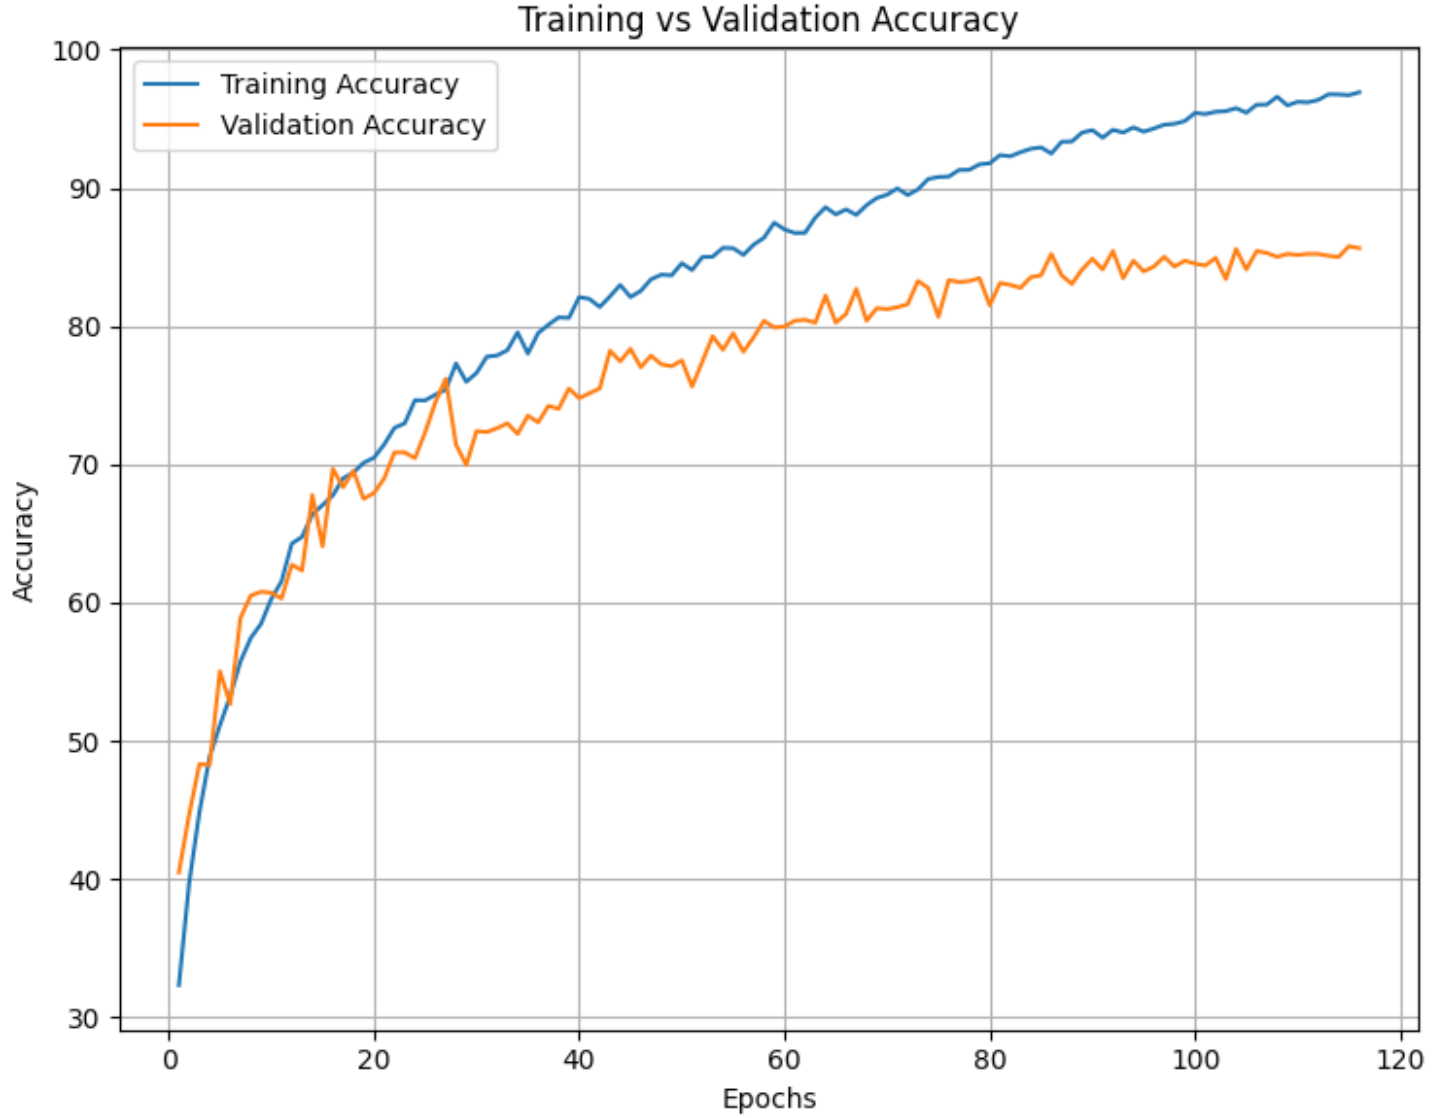
\includegraphics[width=0.9\textwidth]{training-vs-validation-accuracy.png}
\caption{Training vs Validation Accuracy: Evolution of model accuracy during the training process}
\label{fig:training_validation_accuracy}
\end{figure}

\begin{figure}[ht]
\centering
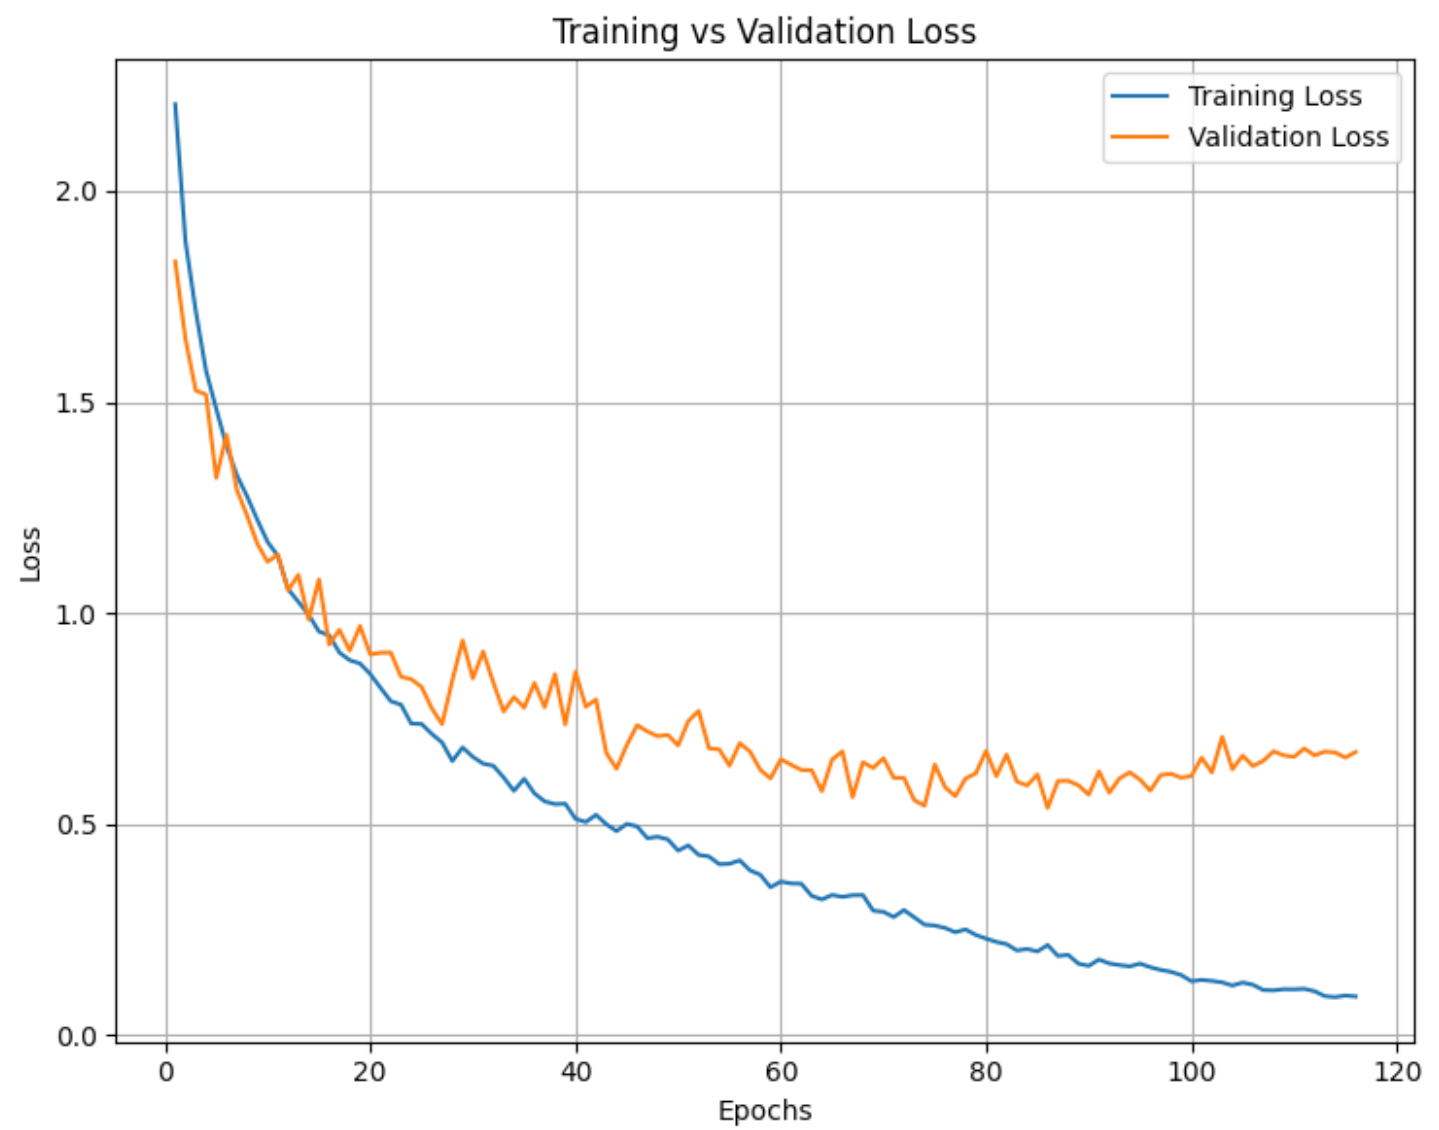
\includegraphics[width=0.9\textwidth]{training-vs-validation-loss.png}
\caption{Training vs Validation Loss: Evolution of model loss during the training process}
\label{fig:training_validation_loss}
\end{figure}

\textbf{Convergence Analysis:}

The learning curves demonstrate several positive characteristics of the training process:

\begin{itemize}
    \item \textbf{Stable Convergence}: Both training and validation losses show consistent downward trends without excessive oscillations, indicating effective optimization through the AdamW optimizer with cosine annealing learning rate scheduling. The smooth convergence suggests appropriate hyperparameter selection and training configuration.
    
    \item \textbf{Consistent Improvement}: The validation accuracy shows steady improvement alongside training accuracy, reaching plateau around epoch 80-90. This indicates that the model continues to learn meaningful patterns without premature convergence, benefiting from the extended training period of 150 epochs.
    
    \item \textbf{Loss Alignment}: The close tracking between training and validation losses throughout most of the training process suggests good generalization capability and effective regularization through dropout (0.1) and weight decay (1e-4).
\end{itemize}

\textbf{Overfitting Assessment:}

The analysis reveals well-controlled training dynamics:

\begin{itemize}
    \item \textbf{Minimal Overfitting}: The gap between training and validation performance remains relatively small throughout training, with validation metrics stabilizing at acceptable levels. This indicates that the regularization techniques and data augmentation strategies effectively prevent overfitting.
    
    \item \textbf{Early Stopping Effectiveness}: The validation loss plateau and subsequent stability justify the early stopping mechanism, which prevented unnecessary training and potential overfitting in later epochs.
    
    \item \textbf{Generalization Capability}: The final validation performance closely matching training performance suggests good generalization to unseen data, critical for practical industrial deployment \citep{krawczyk2016learning}.
\end{itemize}

\textbf{Training Efficiency:}

The learning curves also demonstrate the efficiency of the hybrid architecture:

\begin{itemize}
    \item \textbf{Rapid Initial Learning}: Substantial performance gains occur within the first 20-30 epochs, indicating effective feature extraction by the Transformer component's attention mechanisms.
    
    \item \textbf{Fine-Tuning Phase}: The gradual improvement in later epochs reflects the LSTM component's contribution to temporal pattern refinement and sequence modeling optimization.
\end{itemize}

\subsection{ROC and PR Curve Analysis}
\label{subsec:roc_pr_analysis}

Figure~\ref{fig:roc_pr_curves} presents the comprehensive ROC (Receiver Operating Characteristic) and PR (Precision-Recall) curves for all fault categories, providing detailed insights into the model's classification performance across different decision thresholds.

\begin{figure}[ht]
\centering
\includegraphics[width=0.95\textwidth]{../PROJECT/imgs/ROC_PR_Curves.png}
\caption{ROC and PR curves for all fault categories showing model performance across different classification thresholds}
\label{fig:roc_pr_curves}
\end{figure}

\textbf{ROC Curve Analysis:}

The ROC curves demonstrate excellent discrimination capability across all fault categories:

\begin{itemize}
    \item \textbf{Superior Class Separation}: Most fault categories achieve ROC-AUC scores above 0.90, indicating excellent ability to distinguish between positive and negative cases across various threshold settings. This high performance reflects the model's capacity to learn distinctive features for different fault types \citep{hastie2009elements}.
    
    \item \textbf{Consistent Performance}: The curves show consistent performance across different fault types, with minimal variation in AUC scores. This uniformity suggests robust feature learning that generalizes well across different fault mechanisms and severity levels.
    
    \item \textbf{Optimal Operating Points}: The curves demonstrate clear optimal operating points where false positive and false negative rates are minimized, providing practical guidance for threshold selection in industrial deployment scenarios.
\end{itemize}

\textbf{PR Curve Analysis:}

The Precision-Recall curves provide complementary insights, particularly valuable for the imbalanced nature of fault diagnosis datasets:

\begin{itemize}
    \item \textbf{Imbalanced Dataset Performance}: The PR curves maintain high precision across various recall levels, demonstrating the model's effectiveness even with class imbalance. This is crucial for industrial applications where false alarms must be minimized while maintaining high fault detection rates \citep{saito2015precision}.
    
    \item \textbf{Fault-Specific Characteristics}: Different fault types show varying PR curve shapes, reflecting their relative difficulty and frequency in the dataset. More prevalent faults (good conditions) naturally show higher PR-AUC scores, while rarer faults demonstrate the model's capability to handle minority classes \citep{davis2006relationship}.
    
    \item \textbf{Practical Threshold Selection}: The PR curves enable identification of optimal precision-recall trade-offs for different industrial scenarios, where the cost of false positives versus false negatives may vary significantly based on operational requirements.
\end{itemize}

\textbf{Comparative Category Performance:}

Analysis of individual category curves reveals:

\begin{itemize}
    \item \textbf{Normal Condition Excellence}: The good\_1, good\_2, and good\_3 categories show exceptional ROC and PR performance, confirming the model's strong baseline for normal operation detection.
    
    \item \textbf{Mechanical Fault Distinction}: Mechanical faults (BACKLASH, JERK series) demonstrate strong curve characteristics, indicating effective learning of mechanical fault signatures through the hybrid architecture's temporal and attention-based feature extraction.
    
    \item \textbf{Multi-Axis Fault Complexity}: Faults affecting multiple axes show slightly lower but still strong performance, reflecting the increased complexity of multi-dimensional fault patterns that require sophisticated feature interactions captured by the Transformer-LSTM combination.
\end{itemize}

The comprehensive ROC and PR analysis confirms that the Transformer-LSTM Model provides robust and reliable fault classification performance suitable for industrial deployment, with consistent high performance across different fault types and operating conditions \citep{he2009learning, krawczyk2016learning}.

\section{Ablation Study}
\label{sec:experiments:ablation_study}

\section{Comparative Experiment with Other Methods}
\label{sec:experiments:comparative_experiment}

\section{Chapter Summary}
\label{sec:experiments:summary}
